% !TEX root = ../thesis.tex
\chapter{Tools for Assessing Fairness}
\label{chapter:tools_for_assessing_fairness}
\thispagestyle{empty}

The aim of this chapter is to provide the reader with an overview on the tools adopted in our experiments, recalling the technical concepts addressed in Chapter~\ref{chapter:technical_preliminaries}.

We describe the functioning behind:
\begin{itemize}
\item \textit{The `Glassdoor Method'}, a framework for evaluating gender pay gap which relies on linear regression.
\item \textit{FAIR-DB}, an algorithm based on functional dependencies and the related evaluation metrics.
\item \textit{Ranking Facts}, an application built on the idea of ranking which makes use, among other things, of some of the statistical concepts previously introduced.
\end{itemize}
We are not claiming that the above is an exhaustive list of approaches for discovering bias and assessing fairness in data, but we decided to focus on them because they are recent and provide us with interesting and diversified points of view.


\section{The `Glassdoor Method'}
\label{section:the_glassdoor_method}
After having explored the technical basics in Chapter~\ref{chapter:technical_preliminaries}, we now make an overview of the tools used for this research. The first one is a technical guide to analyze gender pay gap in a company, provided by \textbf{Glassdoor} in \cite{chamberlain2017analyze}.

Glassdoor is a website in which employees and ex-employees of companies anonymously review enterprises and their superiors, with the overall aim of providing insights about jobs and companies and helping people find the most suitable working position for them. The society was founded in 2007 in the U.S. and the website was made available in 2008; since then, the company has grown to become the worldwide leader in the sector.

As specified in the introduction of the guide \cite[p.~2]{chamberlain2017analyze}, according to a 2016 Glassdoor survey, 67\% of the U.S. employees would not apply for jobs at employers where they believe a gender pay gap exists. The purpose of the report is therefore to help HR practitioners in analyzing the internal gender pay gap of their companies, by providing them specific technical knowledge.

First of all, by `gender pay gap' Chamberlain means:
\begin{quote}\emph{The difference between average pay for men and women, both before and after we've accounted for differences among workers in education, experience, job roles, employee performance and other factors aside from gender that affect pay.} \cite[p.~3]{chamberlain2017analyze}\end{quote}
Two measures are proposed in the report, respectively referred as `unadjusted' and `adjusted' pay gap:
\begin{itemize}
\item \textbf{`Unadjusted' pay gap}:
\begin{quote}\emph{Average pay for men as a group, compared to average pay for women as a group.} \cite[p.~3]{chamberlain2017analyze}\end{quote}
Therefore, the formula for estimating `unadjusted' gender pay gap is: \[U = \frac{\mathrm{avg}(BasePay)_m - \mathrm{avg}(BasePay)_f}{\mathrm{avg}(BasePay)_m}\] where \(\mathrm{avg}(BasePay)_m\) is the average pay (arithmetic mean of salaries) of male employees, while \(\mathrm{avg}(BasePay)_f\) is the average pay of female employees.
For the sake of completeness, despite being a basic mathematical concept, we define the \textit{mean} as the sum of a collections of numbers (in this case, salaries) divided by the count of numbers in the collection (the total amount of males or females). Taking \(n\) as total number of male employees: \[\mathrm{avg}(BasePay)_m = \frac{\sum\limits_{i=1}^n BasePay_i}{n}\] and the same holds for female employees.
\item \textbf{`Adjusted' pay gap}: while the `unadjusted' pay gap is basically a simple comparison of all women with all men, the `adjusted' pay gap compares similarly situated male and female employees, in order to include in the calculation the numerous factors that affect the pay (e.g. job title, or educational level). The estimation of the `adjusted' pay gap is based on linear regression, a concept presented in Section~\ref{section:linear_regression}, and the reference formula is: \[y_i = \beta_1\textit{Male}_i + \beta_2X_i + \epsilon_i\] where \(y_i\) is the annual salary of worker \(i\), \(\textit{Male}_i\) is a dummy indicator equal to 1 for males and 0 for females, and \(X_i\) is a collection of attributes of employees which may be relevant for the calculation (job title, educational level, etc.). The estimated coefficient \(\beta_1\) represents the approximate pay advantage for men compared to women.
\end{itemize}


\section{FAIR-DB}
\label{section:fair-db}
The second tool adopted for this research is called \textbf{FAIR-DB} (\textit{\textbf{F}unction\textbf{A}l Dependenc\textbf{I}es to discove\textbf{R} \textbf{D}ata \textbf{B}ias}), and it is a framework with the aim of discovering unfair behaviors in datasets, developed at Politecnico di Milano. As the name itself suggests, FAIR-DB is based on functional dependencies, and it falls within the category of preprocessing techniques since it works by finding conditions (constraints) already present in the data. The developers documented the functioning of FAIR-DB in \cite{azzalini2021fair}, by providing an overview of the tool, together with a clarifying example.

\begin{figure}[t!]
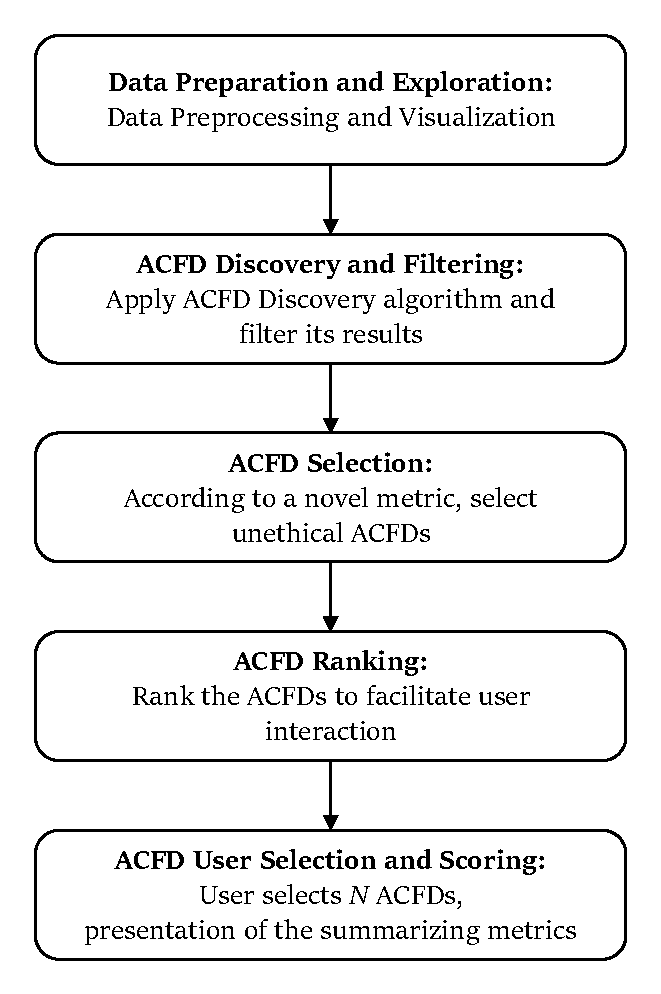
\includegraphics[scale=.65]{figures/fair-db_framework.pdf}
\centering
\caption{Steps of the FAIR-DB framework. Image based on the one shown in \cite{azzalini2021fair}.}
\label{fig:fair-db_framework}
\end{figure}

Figure~\ref{fig:fair-db_framework} shows the framework workflow, while a brief explanation of each phase, as documented in \cite{azzalini2021fair}, is reported below.
\begin{itemize}
\item \textbf{Data preparation and exploration}: data are imported and data integration is eventually performed. Data cleaning, feature selection and discretization techniques are also applied in this phase, in order to deal with missing values, select the smallest set of attributes relevant for the analysis and transform data from numerical to nominal data type. Data are finally plotted in order to help the user in identifying groups in the dataset and eventually majority and minority classes.
\item \textbf{ACFD Discovery and filtering}: the \textit{ACFD Discovery} algorithm, presented in \cite{rammelaere2018revisiting}, is applied to extract approximate conditional functional dependencies from the dataset. The algorithm takes as input the dataset and three threshold parameters: \textit{minimum support}, \textit{minimum confidence} and \textit{maximum antecedent size} of the ACFD sought. From the output, dependencies not involving at least one of the protected attributes and the target attribute (the one used as reference to search for discrimination, e.g. \(\mathit{Income}\)) are removed, as well as dependencies containing variables (in which one or more attributes are not assigned to a specific value, e.g. the attribute \(\mathit{Ideal}\) in \(\mathit{Temperature} = \mlq 28 \mrq, \mathit{pH} = \mlq 7 \mrq \rightarrow \mathit{Ideal}\)).
\item \textbf{ACFD selection}: for each ACFD, some metrics are computed to capture the `ethical level' of the dependency. In particular, the \textit{difference} metric described in Section~\ref{section:evaluation_metrics}, as already mentioned, is a novel score introduced for this purpose, and a second measure called \textit{p-Difference} is calculated for each protected attribute. The p-Difference indicates how much a dependency shows bias with respect to a specific protected attribute, and it is computed in the same way as the difference, but excluding the attribute from the antecedent of the rule. According to the values of the metrics, the most interesting ACFDs are selected.
\item \textbf{ACFD ranking}: the ACFDs are ranked in descending order of importance according to \textit{support}, \textit{difference}, or \textit{mean}. The support emphasize the \textit{pervasiveness} of a rule, because it indicates the number of tuples involved by the dependency, so the higher the value, the more tuples are affected by the ACFD. The difference privileges the \textit{unethical aspect} of a rule, because it highlights dependencies where the values of the protected attributes influence most their RHS. The mean is computed as mean of support and difference, and therefore it gives more importance to the rules with the \textit{best trade-off} between pervasiveness and unethical perspective.
\item \textbf{ACFD user selection and scoring}: the user selects \(N\) ACFDs perceived as the most problematic, and the system computes metrics (based on support, difference, and p-Difference of the selected rules) to summarize the level of unfairness of the dataset.
\end{itemize}


\section{Ranking Facts}
\label{section:ranking_facts}
The third tool used for this research is called \textbf{Ranking Facts}, a Web-based application (of which there also exists a notebook version) developed by the team of \textit{Data, Responsibly}\footnote{Available at: \url{http://demo. dataresponsibly.com/rankingfacts.}}. Ranking Facts, as the name itself suggests, is a \textit{ranking} tool: ranking is an action commonly performed by the vast majority of the algorithms we use every day: Google itself ranks the results of our searches and provides us with a list in descending order of relevance, and the same mechanism is used in various contexts of different nature, like dating or hiring applications. These specific scenarios are particularly relevant, because it is people who are ranked, and therefore discrimination against individuals or protected groups could arise, or the outcome could exhibit low diversity. Ranking Facts is based on the concept of \textit{nutritional labels}, in analogy to the food industry, where simple, standard labels convey information about the ingredients and production processes. Similarly, in the tool nutritional labels are derived as part of the complex process that gave rise to the data or model they describe, embodying the paradigm of interpretability-by-design.

As documented in \cite{yang2018nutritional}, Ranking Facts is a collection of visual widgets with the aim of providing to the user information about the ranking in terms of stability, fairness and diversity. A brief description of how they work, taken from \cite{yang2018nutritional}, is reported below.
\begin{itemize}
\item \textbf{Recipe} and \textbf{Ingredients}: the former widget succinctly describes the ranking algorithm, by listing the attributes used for ranking together with their weights, as specified by the user; while the latter shows, in descending order of importance, the attributes that really affect the ranking.
\item \textbf{Stability}: it explains whether the ranking methodology is robust on the specific dataset in use. An unstable ranking is one where slight changes to the data (e.g. due to uncertainty and noise), or to the methodology (e.g. by slightly adjusting the weights of the attributes in the recipe) could lead to a significant change in the output.
\item \textbf{Fairness}: it quantifies whether the ranked output exhibits statistical parity (group fairness) with respect to one or more protected attributes, such as gender or race of individuals. The notion of fairness is defined specifically for rankings and it can be computed comparing only binary categorical attributes (i.e. non-numerical attributes with just two possible values). The summary view of the widget presents the output of three fairness measures:

\begin{itemize}
\item \textbf{FA*IR} \cite{zehlike2017fa*ir}: ranking algorithm based on the assumption that on a ranking, the desired good for an individual is to appear in the result and to be ranked among the top-\(k\) positions. The outcome is therefore unfair if members of a protected group are systematically ranked lower than those of a privileged group, and a ranking algorithm discriminates unfairly if this ranking decision is based fully or partially on a protected feature.

The \textit{ranked group fairness} criterion used by the algorithm compares the number of protected elements in every prefix of the ranking (i.e. the top-\(i\) positions of the ranking, with \(i \in [1, k]\)) with the expected number of protected elements if they were picked at random using Bernoulli trials (independent `coin tosses') with success probability \(p\). The statistical test also includes a significance parameter \(\alpha\), corresponding to the probability of a type I error, which means rejecting a fair ranking. A clarifying example is provided in Table~\ref{table:fa*ir_example}.

\begin{table}[t!]
\begin{tabularx}{\columnwidth}{|>{\centering\arraybackslash}p{.85cm}|YYYYYYYYYYYY|}
\hline
\diagbox{\(p\)}{\(k\)} & 1 & 2 & 3 & 4 & 5 & 6 & 7 & 8 & 9 & 10 & 11 & 12\\
\hline
0.1 & 0 & 0 & 0 & 0 & 0 & 0 & 0 & 0 & 0 & 0 & 0 & 0\\
0.2 & 0 & 0 & 0 & 0 & 0 & 0 & 0 & 0 & 0 & 0 & 1 & 1\\
0.3 & 0 & 0 & 0 & 0 & 0 & 0 & 1 & 1 & 1 & 1 & 1 & 2\\
0.4 & 0 & 0 & 0 & 0 & 1 & 1 & 1 & 1 & 2 & 2 & 2 & 3\\
0.5 & 0 & 0 & 0 & 1 & 1 & 1 & 2 & 2 & 3 & 3 & 3 & 4\\
0.6 & 0 & 0 & 1 & 1 & 2 & 2 & 3 & 3 & 4 & 4 & 5 & 5\\
0.7 & 0 & 1 & 1 & 2 & 2 & 3 & 3 & 4 & 5 & 5 & 6 & 6\\
\hline
\end{tabularx}
\centering
\caption{Minimum number of candidates in the protected group that must appear in the top-\(k\) positions to pass the ranked group fairness criterion with \(\alpha = 0.1\). Considering for example \(\mathit{gender}\) as a protected attribute with values \(\mlq M \mrq\) and \(\mlq F \mrq\), the minimum number of females (or eventually males) appearing in the top-5 with \(p=0.4\) is \(1\). Table based on the one shown in \cite{zehlike2017fa*ir}.}
\label{table:fa*ir_example}
\end{table}

The algorithm produces a top-\(k\) ranking that satisfies the ranking group fairness criterion mentioned above while maximizing \textit{utility}, which means selecting the `best' tuples, assigning them a score based on the relevant attributes used for the evaluation (e.g. picking the most qualified candidates for a job position by looking at their educational level).

\item \textbf{Proportion} \cite{vzliobaite2017measuring}: this measure is based on the concept of z-test, as described in Section~\ref{section:statistical_concepts}.

\item \textbf{Pairwise}: also known as \textit{pairwise comparison}, it is a tool for prioritizing and ranking multiple options relative to each other. A matrix is generally used to compare each option in pairs and determine which is the preferred choice or has the highest level of importance based on defined criteria. At the end of the comparison process, each option has a rank or relative rating as compared to the rest of the options. Table~\ref{table:pairwise_comparison_example} provides an example: scores are assigned based on how strongly the consumption of a drink on the left dominates that of a drink at the top. For example, when coffee on the left is compared with wine at the top, since coffee appears to be extremely more consumed, 9 is entered in the first row and second column position. A score of $\frac{1}{9}$ is automatically entered in the second row and first column position. According to the matrix, the final ranking would be:\\\(\mathit{Sodas}:~0.252\), \(\mathit{Water}:~0.228\), \(\mathit{Beer}:~0.164\), \(\mathit{Milk}:~0.148\), \(\mathit{Coffee}:~0.142\), \(\mathit{Tea}:~0.046\), \(\mathit{Wine}:~0.019\).

\begin{table}[t!]
\begin{tabularx}{\columnwidth}{|Y|YYYYYYY|}
\hline
& Coffee & Wine & Tea & Beer & Sodas & Milk & Water\\
\hline
Coffee & 1 & 9 & 3 & 1 & $\frac{1}{2}$ & 1 & $\frac{1}{2}$\\
Wine & $\frac{1}{9}$ & 1 & $\frac{1}{3}$ & $\frac{1}{9}$ & $\frac{1}{9}$ & $\frac{1}{9}$ & $\frac{1}{9}$\\
Tea & $\frac{1}{3}$ & 3 & 1 & $\frac{1}{4}$ & $\frac{1}{5}$ & $\frac{1}{4}$ & $\frac{1}{5}$\\
Beer & 1 & 9 & 4 & 1 & $\frac{1}{2}$ & 1 & 1\\
Sodas & 2 & 9 & 5 & 2 & 1 & 2 & 1\\
Milk & 1 & 9 & 4 & 1 & $\frac{1}{2}$ & 1 & $\frac{1}{2}$\\
Water & 2 & 9 & 5 & 1 & 1 & 2 & 1\\
\hline
\end{tabularx}
\centering
\caption{Drink consumption in the U.S. represented in a pairwise comparison matrix. Table based on the one shown in \cite{saaty2003magic}.}
\label{table:pairwise_comparison_example}
\end{table}
\end{itemize}

All these measures are statistical tests, and whether a result is fair is determined by the computed \(p\)-value.
\item \textbf{Diversity}: since fairness is also related to representation, this widget shows diversity with respect to a set of demographic categories of individuals, or a set of categorical attributes of other kinds of items, by displaying the proportion of each category in the top-10 ranked list and overall (i.e. considering all the elements in the ranking).
\end{itemize}
